\documentclass[
	12pt,            % Tamanho da fonte
	openright,       % Capítulos começam em páginas ímpares
	oneside,         % Para impressão em uma face
	a4paper,         % Tamanho do papel A4
	english,         % Idioma secundário
	brazil           % Idioma principal
]{abntex2}

\usepackage{graphicx}          % Para incluir imagens
\usepackage[utf8]{inputenc}    % Codificação UTF-8
\usepackage[T1]{fontenc}       % Encoding para fontes
\usepackage{indentfirst}       % Indenta o primeiro parágrafo de cada seção
\usepackage{microtype}         % Melhorias na justificação do texto
\usepackage{hyperref}          % Links clicáveis
\usepackage{amsmath,amssymb}   % Pacotes matemáticos
\usepackage{wasysym}           % Para símbolos incluindo checkbox
\usepackage{setspace}
\usepackage{float}             % Controle preciso de posicionamento de floats
\usepackage{xcolor}

% Configurações de margens
\usepackage{geometry}

% Configuração de numeração de seções
\renewcommand{\thesection}{\arabic{section}}

\geometry{
	a4paper,
	left=3cm,        % Margem esquerda
	right=2cm,       % Margem direita
	top=3cm,         % Margem superior
	bottom=2cm       % Margem inferior
}

\setlength{\parindent}{1.25cm}  % Recuo da primeira linha do parágrafo
\setlength{\parskip}{0.2cm}     % Espaço entre parágrafos

\usepackage{hyperref}
\begin{document}

\begin{center} 
    Universidade de São Paulo \linebreak
    Faculdade de Filosofia, Ciências e Letras de Ribeirão Preto (FFCLRP) \linebreak
    Departamento de Computação e Matemática (DCM)
    
    \vfill
    
    \Huge Cartas de Amor: um Jogo Distribuído % TÍTULO
    
    \normalsize
    \vfill
    
    % NOMES
    Lucas Cardoso dos Santos (9865492)\\
    Maya Monteiro Lima (13671942)\\
    Miguel de Carvalho Oliveira  (13672172)\\

    \vfill
    
    Ribeirão Preto
    
    2025
    
\end{center} %página1%

\newpage

\tableofcontents

\chapter{Introdução}

O desenvolvimento de jogos digitais envolve desafios que vão desde a modelagem de regras e dinâmicas até a implementação de sistemas robustos e seguros. Este relatório apresenta a criação de uma aplicação web multiplayer inspirada no jogo de cartas Love Letter, abordando desde os conceitos fundamentais do jogo, suas regras e mecânicas, até a materialização dessas ideias em uma solução tecnológica moderna.

A solução proposta explora aspectos de autenticação de usuários, gerenciamento de salas de jogo, comunicação em tempo real e sincronização de estados entre múltiplos participantes. Para garantir uma experiência fluida e segura, foram adotadas práticas de arquitetura em camadas, uso de protocolos adequados para cada tipo de interação e a definição de requisitos funcionais claros, que orientaram o desenvolvimento desde o início.

Além da implementação das funcionalidades essenciais, o projeto contempla o desenho de uma base de dados eficiente, capaz de armazenar informações relevantes sobre usuários, partidas e interações. O resultado é uma plataforma que alia entretenimento, tecnologia e boas práticas de engenharia de software, evidenciando o potencial de aplicações web modernas para proporcionar experiências interativas e seguras aos seus usuários.

\chapter{Requisitos}

\section{Requisitos Funcionais}

\begin{itemize}
    \item \textbf{RF01}: O sistema deve permitir o registro de novos usuários com nome de usuário, e-mail e senha.
    \item \textbf{RF02}: O sistema deve permitir autenticação de usuários e manutenção de sessões seguras.
    \item \textbf{RF03}: Usuários autenticados devem poder criar novas salas de jogo.
    \item \textbf{RF04}: O sistema deve listar salas de jogo disponíveis para entrada.
    \item \textbf{RF05}: Cada sala de jogo deve suportar de 2 a 6 jogadores simultâneos.
    \item \textbf{RF06}: O estado do jogo deve ser sincronizado em tempo real entre todos os jogadores, utilizando WebSockets.
    \item \textbf{RF07}: O sistema deve implementar e aplicar as regras oficiais do jogo \textit{Love Letter}, conforme especificado no Apêndice~\ref{appendix:love-letter}.
    \item \textbf{RF08}: O sistema deve permitir que o usuário exclua sua própria conta.
    \item \textbf{RF09}: O sistema deve permitir que o usuário altere seu nome de usuário.
    \item \textbf{RF10}: O usuário deve poder sair de uma sala de jogo a qualquer momento.
    \item \textbf{RF11}: O usuário não pode participar de múltiplas salas simultaneamente.
    \item \textbf{RF12}: O sistema deve notificar os jogadores quando alguém sair da sala.
    \item \textbf{RF13}: O usuário deve poder acessar as regras do jogo a qualquer momento durante a partida.
    \item \textbf{RF14}: O sistema deve exibir logs de ações do jogo de forma compreensível.
\end{itemize}

\section{Requisitos Não-Funcionais}

\subsection{Desempenho}
\begin{itemize}
    \item \textbf{RNF01}: A latência da comunicação em tempo real deve ser inferior a 1 segundo durante as partidas.
    \item \textbf{RNF02}: O sistema deve suportar pelo menos 10 usuários simultâneos sem degradação perceptível de desempenho.
    \item \textbf{RNF03}: O usuário deve poder desabilitar animações para melhorar a performance em dispositivos menos potentes.
\end{itemize}

\subsection{Segurança}
\begin{itemize}
    \item \textbf{RNF04}: Senhas devem ser armazenadas utilizando algoritmos de hash seguros (ex: bcrypt, Argon2).
    \item \textbf{RNF05}: Toda comunicação entre cliente e servidor deve ser criptografada (HTTPS/WSS).
    \item \textbf{RNF06}: Sessões de usuários devem expirar após um período e utilizar tokens de autenticação seguros.
\end{itemize}

\subsection{Usabilidade e Acessibilidade}
\begin{itemize}
    \item \textbf{RNF07}: O sistema deve ser acessível, suportando navegação por teclado e leitores de tela.
    \item \textbf{RNF08}: O sistema deve estar disponível em, pelo menos, português e inglês.
\end{itemize}

\subsection{Portabilidade e Manutenção}
\begin{itemize}
    \item \textbf{RNF09}: O sistema deve funcionar nos principais navegadores modernos (Chrome, Firefox, Edge, Safari) e sistemas operacionais (Windows, Linux, macOS).
    \item \textbf{RNF10}: O código deve seguir princípios de design modular, com documentação e comentários adequados.
    \item \textbf{RNF11}: O sistema deve possuir mecanismos de logging e monitoramento para facilitar manutenção e auditoria.
\end{itemize}

\subsection{Confiabilidade}
\begin{itemize}
    \item \textbf{RNF12}: A sincronização do estado do jogo deve ser testada quanto à consistência e tolerância a falhas de conexão.
    \item \textbf{RNF13}: O sistema deve permitir recuperação de sessões em caso de desconexão temporária.
\end{itemize}

\chapter{Arquitetura do Sistema}

O sistema desenvolvido adota uma arquitetura moderna e robusta, composta por dois principais componentes: um cliente web desenvolvido com Svelte e um servidor backend implementado em .NET. A comunicação entre cliente e servidor é realizada predominantemente via protocolo HTTP para operações tradicionais de gerenciamento (como criação e entrada em salas de jogo, gerenciamento de contas de usuário e obtenção de dados do jogo). Para operações em tempo real, essenciais para a dinâmica do jogo (como jogar cartas, comprar cartas e receber atualizações instantâneas), utiliza-se o protocolo WebSocket, garantindo baixa latência e interatividade.

\section{Arquitetura em Camadas do Backend}
O backend segue o padrão de arquitetura em camadas, promovendo separação de responsabilidades, facilidade de manutenção e escalabilidade. As principais camadas são:

\begin{itemize}
    \item \textbf{Apresentação}: Responsável por expor as APIs HTTP e WebSocket, recebendo e respondendo às requisições dos clientes. Realiza validações iniciais e orquestra o fluxo das operações.
    \item \textbf{Aplicação}: Contém a lógica de orquestração dos casos de uso do sistema, coordenando as operações entre as demais camadas. Implementa os fluxos de negócio sem se preocupar com detalhes de infraestrutura ou regras de domínio.
    \item \textbf{Domínio}: Abriga as regras de negócio centrais e entidades do sistema. É independente de detalhes técnicos e representa o núcleo lógico da aplicação.
    \item \textbf{Infraestrutura}: Implementa detalhes técnicos como persistência de dados, integração com serviços externos e mecanismos de comunicação. Fornece implementações concretas para interfaces definidas nas camadas superiores.
\end{itemize}

\begin{figure}[H]
    \centering
    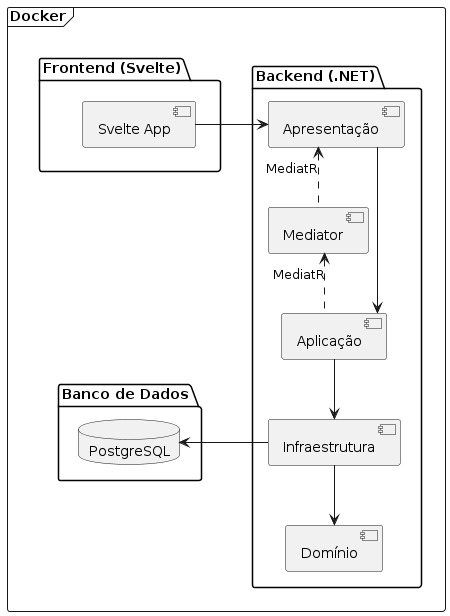
\includegraphics[width=0.7\textwidth]{diagrams/Architecture.png}
    \caption{Diagrama de arquitetura do sistema. Fonte: os autores}
    \label{fig:architecture}
\end{figure}

\section{Padrões de Projeto Utilizados}
O sistema faz uso de alguns padrões de projeto consagrados para promover flexibilidade e desacoplamento:

\begin{enumerate}
    \item \textbf{Repository}: Abstrai o acesso a dados, permitindo que a lógica de negócio interaja com repositórios de forma independente da tecnologia de persistência.
    \item \textbf{Mediator}: Centraliza a comunicação entre componentes, facilitando a implementação de casos de uso e reduzindo o acoplamento entre objetos.
    \item \textbf{Factory}: Facilita a criação de objetos complexos, encapsulando a lógica de instanciação e promovendo flexibilidade na escolha de implementações.
\end{enumerate}

Essa arquitetura garante que o sistema seja modular, testável e preparado para evoluções futuras.

\section{Arquitetura do Frontend}
O frontend do sistema foi desenvolvido utilizando o framework Svelte, que permite a criação de interfaces web reativas e eficientes. A estrutura do projeto segue boas práticas de modularização e separação de responsabilidades, facilitando a manutenção e a escalabilidade da aplicação.

O código-fonte do frontend está organizado em componentes Svelte, cada um responsável por uma parte específica da interface do usuário, como telas de login, gerenciamento de salas, lobby, mesa de jogo e exibição de cartas. Essa abordagem baseada em componentes permite o reuso de código e a fácil evolução da interface.

Além disso, o frontend faz uso de stores reativos do Svelte para gerenciar o estado global da aplicação, como informações do usuário autenticado, estado da sala e dados da partida em andamento. Isso garante que as atualizações de estado sejam refletidas automaticamente na interface, proporcionando uma experiência fluida ao usuário.

A arquitetura adotada no frontend, aliada ao uso de Svelte, resulta em uma aplicação leve, responsiva e de fácil manutenção, preparada para futuras expansões e melhorias.

\section{Tecnologias Utilizadas}
Durante o desenvolvimento do sistema, foram empregadas diversas tecnologias que contribuíram para a robustez, escalabilidade e facilidade de manutenção da solução:

\begin{itemize}
    \item \textbf{SignalR}: Utilizado para facilitar a comunicação em tempo real via WebSocket entre servidor e clientes. O SignalR abstrai a complexidade do gerenciamento de conexões, transmissão de mensagens e reconexão automática, permitindo implementar funcionalidades interativas e síncronas de forma simples e eficiente.
    \item \textbf{MediatR}: Biblioteca empregada para implementar o padrão Mediator no backend, promovendo o desacoplamento entre as camadas de Apresentação e Aplicação. O MediatR centraliza o envio e o tratamento de comandos, queries e eventos, facilitando a manutenção e a evolução do código.
    \item \textbf{PostgreSQL e Entity Framework}: O sistema utiliza o banco de dados relacional PostgreSQL para persistência dos dados, integrado ao backend por meio do Entity Framework, que provê uma camada de abstração para o acesso e manipulação dos dados de forma orientada a objetos.
    \item \textbf{Docker}: Utilizado para empacotar e distribuir tanto o backend quanto o frontend em containers, garantindo portabilidade, reprodutibilidade e facilidade de deploy em diferentes ambientes.
\end{itemize}

Essas tecnologias, integradas à arquitetura do sistema, proporcionam uma base sólida para o desenvolvimento, operação e evolução contínua da aplicação.

\chapter{Funcionamento do Sistema}

O sistema Love Letter é uma aplicação web multiplayer que permite aos usuários jogar o jogo de cartas Love Letter em tempo real através de seus navegadores. O funcionamento do sistema pode ser compreendido através de diferentes perspectivas: o fluxo de interação do usuário, a arquitetura técnica, e os mecanismos de sincronização em tempo real.

\section{Fluxo de Interação do Usuário}

\subsection{Autenticação e Gerenciamento de Conta}
O usuário inicia sua experiência criando uma conta ou fazendo login no sistema. O processo de autenticação utiliza tokens JWT para manter a sessão do usuário de forma segura. Após a autenticação, o usuário tem acesso ao dashboard principal, onde pode gerenciar seu perfil, visualizar salas disponíveis ou criar novas salas de jogo.

\subsection{Criação e Entrada em Salas}
O usuário pode criar uma nova sala de jogo, definindo um nome e opcionalmente uma senha para acesso restrito. Alternativamente, pode visualizar todas as salas disponíveis e entrar em uma delas. O sistema suporta até seis jogadores por sala, e cada sala possui um host (criador) que tem permissões especiais, como a capacidade de deletar a sala.

\subsection{Início da Partida}
Uma vez na sala, os jogadores aguardam o início da partida. O host pode iniciar o jogo quando houver pelo menos dois jogadores presentes. O sistema automaticamente distribui as cartas iniciais e determina a ordem de jogo, iniciando com o primeiro jogador, conforme ilustrado na Figura~\ref{fig:start-game-flow}.

\begin{figure}[h]
    \centering
    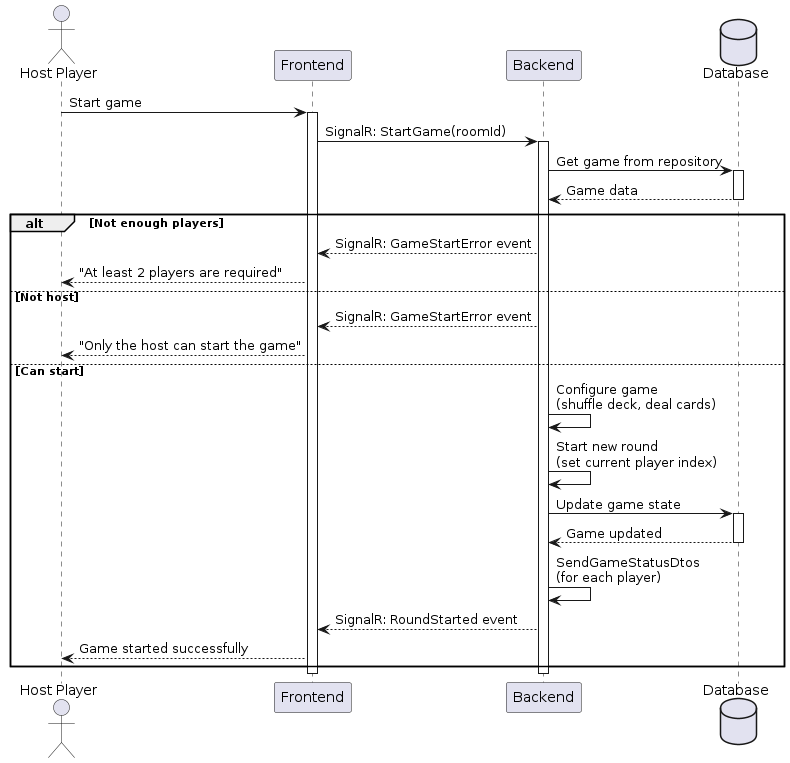
\includegraphics[width=0.8\textwidth]{diagrams/StartGame.png}
    \caption{Fluxo de início do jogo. Fonte: os autores}
    \label{fig:start-game-flow}
\end{figure}

A Figura~\ref{fig:start-game-flow} ilustra o processo de início do jogo. O host solicita o início da partida através da interface, o que dispara uma mensagem SignalR para o servidor. O sistema então valida se há jogadores suficientes (mínimo de 2) e se o solicitante é realmente o host da sala. Se todas as validações passarem, o sistema configura o jogo embaralhando o baralho, distribuindo as cartas iniciais e definindo o primeiro jogador. O estado do jogo é atualizado no banco de dados e todos os jogadores são notificados do início da rodada.

\section{Mecanismos de Jogo}

\subsection{Ciclo de Turno}
O jogo segue um ciclo de turnos bem definido:

\begin{enumerate}
    \item \textbf{Compra de Carta}: O jogador da vez compra uma carta do baralho, adicionando-a à sua mão
    \item \textbf{Jogada de Carta}: O jogador escolhe uma das duas cartas em sua mão para jogar, executando seu efeito específico
    \item \textbf{Resolução de Efeitos}: O sistema processa o efeito da carta jogada, que pode incluir eliminação de jogadores, proteção, troca de cartas, entre outros
    \item \textbf{Avanço de Turno}: O turno passa para o próximo jogador ativo
\end{enumerate}

O diagrama da Figura~\ref{fig:game-turn-flow} ilustra o fluxo geral dessas etapas durante um turno.

\begin{figure}[h]
    \centering
    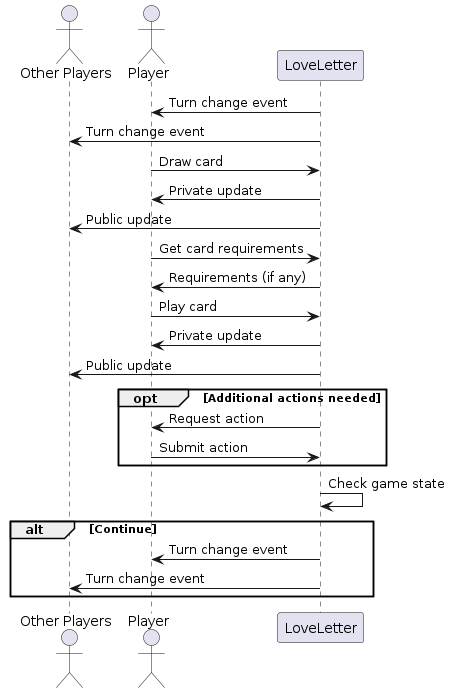
\includegraphics[width=0.4\textwidth]{diagrams/GameTurnFlow.png}
    \caption{Fluxo geral de um turno no jogo. Fonte: os autores}
    \label{fig:game-turn-flow}
\end{figure}

A Figura~\ref{fig:advance-turn-flow} ilustra o processo de verificação de finalização tanto de rodadas quanto do jogo completo. Após cada jogada, o sistema verifica se a rodada terminou (por eliminação de jogadores ou esgotamento do baralho). Se a rodada terminou, o sistema determina os vencedores e concede pontos bônus quando aplicável. Em seguida, verifica se o jogo completo terminou (quando um jogador atinge a pontuação necessária). Se o jogo não terminou, uma nova rodada é iniciada com a distribuição de novas cartas. Caso contrário, o turno simplesmente avança para o próximo jogador ativo.

\begin{figure}[h]
    \centering
    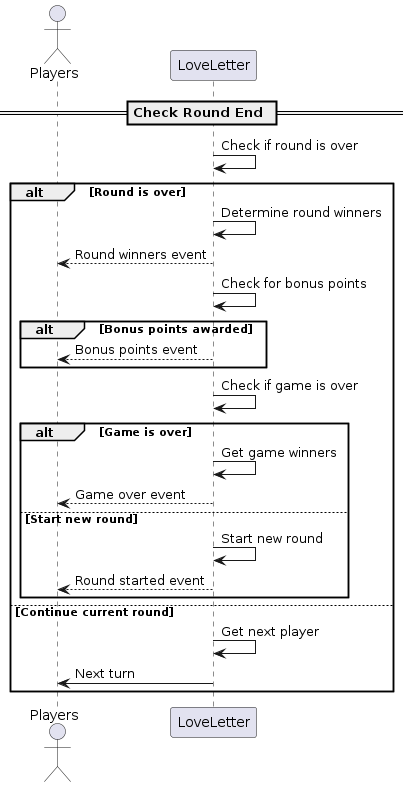
\includegraphics[width=0.35\textwidth]{diagrams/AdvanceTurnFlow.png}
    \caption{Fluxo de avanço de turno e verificação de finalização. Fonte: os autores}
    \label{fig:advance-turn-flow}
\end{figure}

\subsection{Sistema de Cartas}
O jogo utiliza 10 tipos diferentes de cartas, cada uma com valores e efeitos únicos, conforme ilustrado nas Figuras~\ref{fig:spy-card-play} a~\ref{fig:princess-card-play}:

\begin{itemize}
    \item \textbf{Espião (0)}: Concede ponto bônus se mantido até o final da rodada
    \item \textbf{Guarda (1)}: Permite adivinhar a carta de outro jogador
    \item \textbf{Padre (2)}: Permite olhar a carta de outro jogador
    \item \textbf{Barão (3)}: Compara cartas com outro jogador
    \item \textbf{Criada (4)}: Protege o jogador até seu próximo turno
    \item \textbf{Príncipe (5)}: Força outro jogador a descartar e comprar nova carta
    \item \textbf{Chanceler (6)}: Permite comprar duas cartas e escolher qual manter
    \item \textbf{Rei (7)}: Troca cartas com outro jogador
    \item \textbf{Condessa (8)}: Deve ser jogada quando o jogador possui Rei ou Príncipe
    \item \textbf{Princesa (9)}: Elimina o jogador se descartada
\end{itemize}

% Espião (0) e Guarda (1)
\begin{figure}[h]
    \centering
    \begin{minipage}{0.48\textwidth}
        \centering
        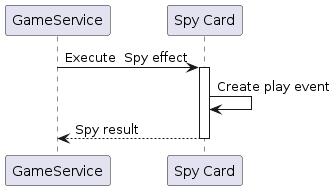
\includegraphics[width=\textwidth]{diagrams/SpyCardPlay.png}
        \caption{Jogada da carta Espião. Fonte: os autores}
        \label{fig:spy-card-play}
    \end{minipage}
    \hfill
    \begin{minipage}{0.48\textwidth}
        \centering
        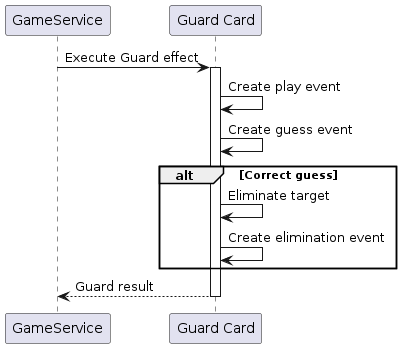
\includegraphics[width=\textwidth]{diagrams/GuardCardPlay.png}
        \caption{Jogada da carta Guarda. Fonte: os autores}
        \label{fig:guard-card-play}
    \end{minipage}
\end{figure}

% Sacerdote (2) e Barão (3)
\begin{figure}[h]
    \centering
    \begin{minipage}{0.48\textwidth}
        \centering
        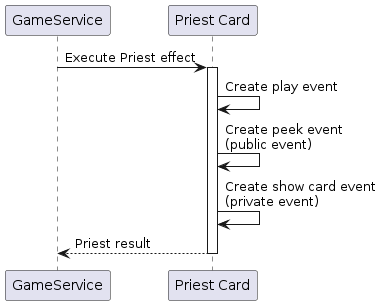
\includegraphics[width=\textwidth]{diagrams/PriestCardPlay.png}
        \caption{Jogada da carta Sacerdote. Fonte: os autores}
        \label{fig:priest-card-play}
    \end{minipage}
    \hfill
    \begin{minipage}{0.48\textwidth}
        \centering
        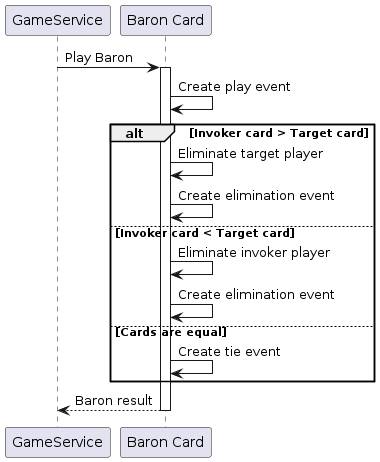
\includegraphics[width=\textwidth]{diagrams/BaronCardPlay.png}
        \caption{Jogada da carta Barão. Fonte: os autores}
        \label{fig:baron-card-play}
    \end{minipage}
\end{figure}

% Criada (4) e Príncipe (5)
\begin{figure}[h]
    \centering
    \begin{minipage}{0.48\textwidth}
        \centering
        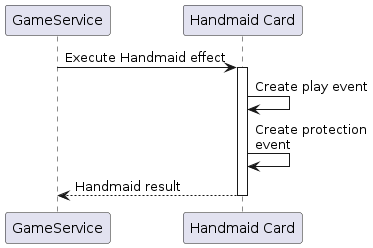
\includegraphics[width=\textwidth]{diagrams/HandmaidCardPlay.png}
        \caption{Jogada da carta Criada. Fonte: os autores}
        \label{fig:handmaid-card-play}
    \end{minipage}
    \hfill
    \begin{minipage}{0.48\textwidth}
        \centering
        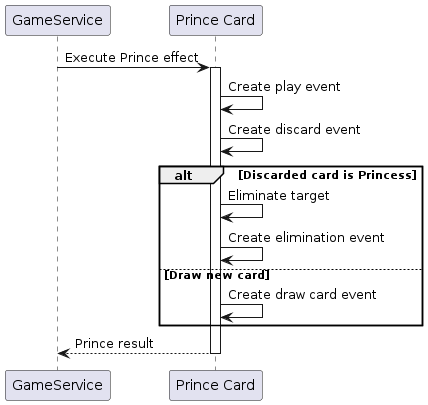
\includegraphics[width=\textwidth]{diagrams/PrinceCardPlay.png}
        \caption{Jogada da carta Príncipe. Fonte: os autores}
        \label{fig:prince-card-play}
    \end{minipage}
\end{figure}

% Chanceler (6) e Rei (7)
\begin{figure}[h]
    \centering
    \begin{minipage}{0.48\textwidth}
        \centering
        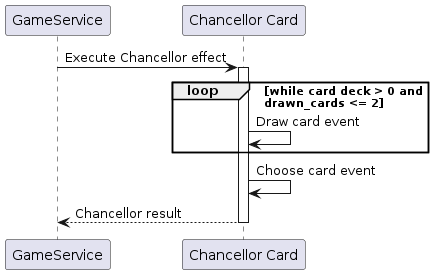
\includegraphics[width=\textwidth]{diagrams/ChancellorCardPlay.png}
        \caption{Jogada da carta Chanceler. Fonte: os autores}
        \label{fig:chancellor-card-play}
    \end{minipage}
    \hfill
    \begin{minipage}{0.48\textwidth}
        \centering
        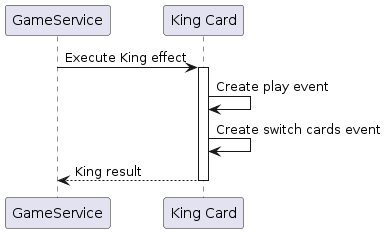
\includegraphics[width=\textwidth]{diagrams/KingCardPlay.png}
        \caption{Jogada da carta Rei. Fonte: os autores}
        \label{fig:king-card-play}
    \end{minipage}
\end{figure}

% Condessa (8) e Princesa (9)
\begin{figure}[h]
    \centering
    \begin{minipage}{0.48\textwidth}
        \centering
        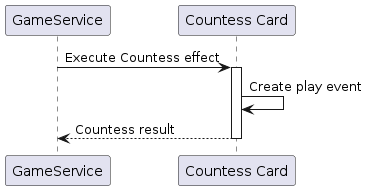
\includegraphics[width=\textwidth]{diagrams/CountessCardPlay.png}
        \caption{Jogada da carta Condessa. Fonte: os autores}
        \label{fig:countess-card-play}
    \end{minipage}
    \hfill
    \begin{minipage}{0.48\textwidth}
        \centering
        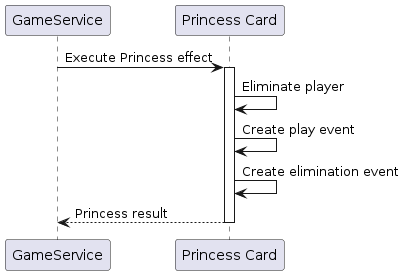
\includegraphics[width=\textwidth]{diagrams/PrincessCardPlay.png}
        \caption{Jogada da carta Princesa. Fonte: os autores}
        \label{fig:princess-card-play}
    \end{minipage}
\end{figure}

\subsection{Estados do Jogo}
O sistema gerencia diferentes estados do jogo para garantir que as ações sejam executadas na ordem correta:

\begin{itemize}
    \item \textbf{WaitingForPlayers}: Aguardando jogadores entrarem na sala
    \item \textbf{WaitingForDraw}: Aguardando o jogador da vez comprar uma carta
    \item \textbf{WaitingForPlay}: Aguardando o jogador escolher e jogar uma carta
    \item \textbf{Finished}: Jogo finalizado
\end{itemize}

\section{Validação de Ações}

O sistema implementa múltiplas camadas de validação para garantir que apenas ações válidas sejam executadas:

\begin{itemize}
    \item \textbf{Validação de Turno}: Apenas o jogador da vez pode executar ações
    \item \textbf{Validação de Estado}: Ações só são permitidas nos estados apropriados do jogo
    \item \textbf{Validação de Cartas}: O jogador deve possuir a carta que deseja jogar
    \item \textbf{Validação de Requisitos}: Cartas com efeitos específicos requerem parâmetros adicionais
\end{itemize}

\section{Experiência do Usuário}

\subsection{Interface Responsiva}
O frontend desenvolvido em Svelte oferece uma interface moderna e responsiva, com animações suaves que podem ser desabilitadas para melhorar a performance em dispositivos menos potentes.

\subsection{Feedback Visual}
O sistema fornece feedback visual claro para todas as ações:

\begin{itemize}
    \item \textbf{Indicadores de Turno}: Mostra claramente de quem é a vez
    \item \textbf{Log de Jogo}: Mantém histórico de todas as ações executadas
    \item \textbf{Animações de Cartas}: Visualiza movimentação e efeitos das cartas
    \item \textbf{Notificações de Estado}: Informa mudanças importantes no jogo
\end{itemize}

\subsection{Acessibilidade}
O sistema inclui recursos de acessibilidade como:

\begin{itemize}
    \item \textbf{Suporte a Múltiplos Idiomas}: Interface disponível em português, inglês e espanhol
    \item \textbf{Controles Intuitivos}: Interface clara e fácil de navegar
\end{itemize}

Esta arquitetura garante que o sistema Love Letter ofereça uma experiência de jogo fluida, segura e envolvente para todos os participantes, mantendo a fidelidade às regras originais do jogo enquanto aproveita as capacidades da tecnologia moderna para criar uma experiência multiplayer online robusta.

\chapter{Endpoints da Aplicação}

\section{Endpoints HTTP}

Abaixo estão listados os principais endpoints HTTP disponíveis na API do backend, organizados por funcionalidade:

% --- Gerenciamento de Conta ---

% Autenticação: Os endpoints que requerem autenticação utilizam JWT Bearer Token, enviado no header Authorization: Bearer <token>.

\subsection{Gerenciamento de Conta}
\begin{itemize}
    \item \textbf{POST /api/Account/create}
    \begin{itemize}
        \item Cria uma nova conta de usuário.
        \item \textbf{Requer autenticação?} Não
        \item \textbf{Body:} username, email, password
        \item \textbf{Retorno:} 200 (token de acesso e mensagem de sucesso), 409 (usuário já existe)
    \end{itemize}
    \item \textbf{POST /api/Account/login}
    \begin{itemize}
        \item Realiza login do usuário.
        \item \textbf{Requer autenticação?} Não
        \item \textbf{Body:} email, password
        \item \textbf{Retorno:} 200 (token de acesso), 401 (credenciais inválidas)
    \end{itemize}
    \item \textbf{PUT /api/Account/{email}}
    \begin{itemize}
        \item Atualiza os dados da conta do usuário autenticado.
        \item \textbf{Requer autenticação?} Sim (JWT Bearer Token)
        \item \textbf{Body:} username
        \item \textbf{Retorno:} 200 (sucesso), 401 (não autenticado), 403 (proibido), 404 (usuário não encontrado)
    \end{itemize}
    \item \textbf{DELETE /api/Account/{email}}
    \begin{itemize}
        \item Deleta a conta do usuário autenticado.
        \item \textbf{Requer autenticação?} Sim (JWT Bearer Token)
        \item \textbf{Retorno:} 200 (sucesso), 401 (não autenticado), 403 (proibido), 404 (usuário não encontrado)
    \end{itemize}
\end{itemize}

% --- Salas de Jogo ---

\subsection{Salas de Jogo}
\begin{itemize}
    \item \textbf{POST /api/GameRoom}
    \begin{itemize}
        \item Cria uma nova sala de jogo.
        \item \textbf{Requer autenticação?} Sim (JWT Bearer Token)
        \item \textbf{Body:} nome da sala, senha (opcional)
        \item \textbf{Retorno:} 200 (ID da sala), 400 (erro de validação), 500 (erro interno)
    \end{itemize}
    \item \textbf{GET /api/GameRoom}
    \begin{itemize}
        \item Lista todas as salas de jogo disponíveis.
        \item \textbf{Requer autenticação?} Sim (JWT Bearer Token)
        \item \textbf{Retorno:} 200 (lista de salas), 500 (erro interno)
    \end{itemize}
    \item \textbf{GET /api/GameRoom/user}
    \begin{itemize}
        \item Lista as salas em que o usuário autenticado está participando.
        \item \textbf{Requer autenticação?} Sim (JWT Bearer Token)
        \item \textbf{Retorno:} 200 (lista de salas do usuário), 500 (erro interno)
    \end{itemize}
    \item \textbf{DELETE /api/GameRoom/{roomId}}
    \begin{itemize}
        \item Deleta uma sala de jogo (se o usuário for o host).
        \item \textbf{Requer autenticação?} Sim (JWT Bearer Token)
        \item \textbf{Retorno:} 204 (sucesso), 404 (sala não encontrada ou não autorizado), 500 (erro interno)
    \end{itemize}
\end{itemize}

% --- Saúde da Aplicação ---

\subsection{Saúde da Aplicação}
\begin{itemize}
    \item \textbf{GET /Health}
    \begin{itemize}
        \item Verifica se a aplicação está funcionando corretamente.
        \item \textbf{Requer autenticação?} Não
        \item \textbf{Retorno:} 200 (status e timestamp)
    \end{itemize}
\end{itemize}

\section{Mensagens WebSocket (SignalR)}

A aplicação utiliza WebSocket via SignalR para comunicação em tempo real durante as partidas. Abaixo estão listadas as principais mensagens (eventos) trocadas entre cliente e servidor, organizadas por funcionalidade:

\subsection{Mensagens Recebidas do Servidor}
\begin{itemize}
    \item \textbf{JoinedRoom}: Confirmação de entrada em uma sala de jogo.
    \item \textbf{UserJoined}: Notifica que um novo jogador entrou na sala.
    \item \textbf{UserLeft}: Notifica que um jogador saiu da sala.
    \item \textbf{UsernameChanged}: Informa alteração de nome de usuário de um participante.
    \item \textbf{RoundStarted}: Início de uma nova rodada.
    \item \textbf{CurrentGameStatus}: Atualização do estado atual da partida.
    \item \textbf{NextTurn}: Indica de quem é a vez de jogar.
    \item \textbf{PlayerDrewCard}: Notifica que um jogador comprou uma carta.
    \item \textbf{GameStartError}: Erro ao tentar iniciar a partida.
    \item \textbf{PlayerUpdatePrivate}: Atualização privada do estado do jogador (cartas na mão, etc).
    \item \textbf{DrawCardError}: Erro ao tentar comprar carta.
    \item \textbf{CardRequirements}: Informa requisitos para jogar determinada carta.
    \item \textbf{PlayCardError}: Erro ao tentar jogar uma carta.
    % Eventos de ações de cartas
    \item \textbf{PlayCard}: Alguém jogou uma carta (tipo e jogador).
    \item \textbf{GuessCard}: Alguém fez uma tentativa de adivinhar carta de outro jogador.
    \item \textbf{PeekCard}: Alguém olhou a carta de outro jogador.
    \item \textbf{ShowCard}: Uma carta foi revelada.
    \item \textbf{CompareCards}: Comparação de cartas entre jogadores.
    \item \textbf{ComparisonTie}: Empate na comparação de cartas.
    \item \textbf{DiscardCard}: Um jogador descartou uma carta.
    \item \textbf{DrawCard}: Um jogador comprou uma carta.
    \item \textbf{CardReturnedToDeck}: Cartas devolvidas ao baralho.
    \item \textbf{PlayerEliminated}: Um jogador foi eliminado.
    \item \textbf{SwitchCards}: Troca de cartas entre jogadores.
    \item \textbf{PlayerProtected}: Jogador protegido por efeito de carta.
    \item \textbf{ChooseCard}: Jogador deve escolher uma carta.
    % Atualizações públicas
    \item \textbf{PublicPlayerUpdate}: Atualização pública do estado de um jogador.
    % Outros eventos de jogo
    \item \textbf{CardChoiceSubmitted}: Jogador submeteu escolha de carta.
    \item \textbf{CardChoiceError}: Erro ao submeter escolha de carta.
    \item \textbf{MandatoryCardPlay}: Jogada obrigatória de carta específica.
    \item \textbf{RoundWinners}: Fim de rodada, vencedores.
    \item \textbf{BonusPoints}: Jogadores que receberam pontos bônus.
    \item \textbf{GameOver}: Fim de jogo, vencedores.
\end{itemize}

\subsection{Mensagens Enviadas ao Servidor}
\begin{itemize}
    \item \textbf{JoinRoom}: Entrar em uma sala de jogo (parâmetros: roomId, senha).
    \item \textbf{LeaveRoom}: Sair da sala de jogo.
    \item \textbf{ReconnectToRoom}: Reconectar-se a uma sala.
    \item \textbf{StartGame}: Iniciar a partida.
    \item \textbf{DrawCard}: Comprar carta.
    \item \textbf{GetCardRequirements}: Solicitar requisitos para jogar uma carta.
    \item \textbf{PlayCard}: Jogar uma carta (parâmetros: tipo, alvo, etc).
    \item \textbf{SubmitCardChoice}: Submeter escolha de carta após efeitos especiais.
    \item \textbf{GetCurrentGameStatus}: Solicitar status atual da partida.
\end{itemize}

Cada mensagem pode conter parâmetros específicos, conforme a ação desejada. Essas mensagens permitem a sincronização em tempo real do estado do jogo entre todos os participantes.



\chapter{Tabelas da Base de Dados}

\section{Visão Geral das Tabelas}
A base de dados do sistema é composta por três tabelas principais: \textbf{Users}, \textbf{Games} e \textbf{Players}. A seguir, detalhamos cada uma delas:

\subsection{Tabela Users}
\begin{itemize}
    \item \textbf{Email}: identificador único do usuário (chave primária).
    \item \textbf{Username}: nome de exibição do usuário.
    \item \textbf{PasswordHash}: senha do usuário armazenada de forma segura (hash).
\end{itemize}

\subsection{Tabela Games}
\begin{itemize}
    \item \textbf{Id}: identificador único da partida (UUID, chave primária).
    \item \textbf{Name}: nome da partida.
    \item \textbf{HostEmail}: email do usuário que criou a partida (chave estrangeira para Users).
    \item \textbf{Password}: senha da sala (opcional).
    \item \textbf{MaxTokens}: número máximo de tokens para vencer.
    \item \textbf{GameState}: estado atual da partida (ex: aguardando, em andamento, finalizada).
    \item \textbf{CurrentPlayerIndex}: índice do jogador da vez.
    \item \textbf{CardsDeck}: baralho de cartas da partida (array de inteiros).
    \item \textbf{ReservedCard}: carta reservada.
    \item \textbf{CreatedAt} / \textbf{UpdatedAt}: datas de criação e atualização.
\end{itemize}
\textbf{Relações:}
\begin{itemize}
    \item \textbf{HostEmail} referencia Users.
    \item Relação 1:N com Players (uma partida possui vários jogadores).
\end{itemize}

\subsection{Tabela Players}
\begin{itemize}
    \item \textbf{GameId}: identificador da partida (chave primária composta).
    \item \textbf{UserEmail}: email do usuário (chave primária composta).
    \item \textbf{Id}: identificador interno do jogador na partida.
    \item \textbf{HoldingCards}: cartas na mão do jogador (array de inteiros).
    \item \textbf{PlayedCards}: cartas já jogadas pelo jogador (array de inteiros).
    \item \textbf{Score}: pontuação do jogador.
    \item \textbf{Status}: status do jogador na partida (ex: ativo, eliminado).
\end{itemize}
\textbf{Relações:}
\begin{itemize}
    \item \textbf{GameId} referencia Games.
    \item \textbf{UserEmail} referencia Users.
\end{itemize}

Essas tabelas e seus relacionamentos garantem o controle de usuários, partidas e jogadores, permitindo o gerenciamento eficiente do jogo e suas regras.



\appendix
\chapter{Regras do Jogo}\label{appendix:love-letter}
\section{Visão Geral}
Love Letter é um jogo de dedução, risco e eliminação onde os jogadores competem para entregar uma carta de amor à princesa. Cada carta tem um valor diferente e habilidades especiais que podem ajudar ou atrapalhar os jogadores. É um jogo de cartas jogado com 2 a 6 jogadores. O objetivo é vencer um certo número de rodadas (tokens de afeição) sendo o último jogador restante ou segurando a carta de maior valor ao final de uma rodada.

\section{Fluxo do Jogo}
\begin{itemize}
    \item Cada jogador começa com uma carta.
    \item Em seu turno, o jogador compra uma carta e escolhe uma das duas cartas para jogar.
    \item O efeito da carta jogada é aplicado imediatamente.
    \item Jogadores podem ser eliminados durante a rodada com base nos efeitos das cartas.
    \item A rodada termina quando resta apenas um jogador ou quando o baralho acaba.
    \item O jogador com a carta de maior valor vence a rodada.
\end{itemize}

\section{Lista de Cartas e Efeitos}
\begin{itemize}
    \item \textbf{Spy (0)}: Ao final da rodada, se o jogador for o \emph{único} restante que jogou ou descartou um Spy durante aquela rodada, recebe 1 token de afeição, mesmo que não tenha vencido a rodada.
    \item \textbf{Guard (1)}: Adivinhe a carta na mão de outro jogador (exceto Guard). Se acertar, o jogador é eliminado.
    \item \textbf{Priest (2)}: Veja a carta na mão de outro jogador.
    \item \textbf{Baron (3)}: Compare a mão com outro jogador; quem tiver a carta de menor valor é eliminado.
    \item \textbf{Handmaid (4)}: Proteção contra todos os efeitos até seu próximo turno.
    \item \textbf{Prince (5)}: Escolha qualquer jogador (inclusive você) para descartar a mão (revelando a carta, mas sem aplicar seus efeitos) e comprar uma nova carta.
    \item \textbf{Chancellor (6)}: Compre 2 cartas e escolha apenas uma das três cartas na mão para manter. As outras duas cartas retornam ao final do baralho.
    \item \textbf{King (7)}: Troque de mão com outro jogador.
    \item \textbf{Countess (8)}: Deve ser jogada se estiver na mão junto com Prince ou King.
    \item \textbf{Princess (9)}: Se descartada ou jogada, o jogador é eliminado.
\end{itemize}

\section{Como Vencer o Jogo}

Um jogador ganha um token de afeição a cada rodada vencida. O número de tokens necessários para vencer depende do número de jogadores, conforme a tabela abaixo:

\begin{center}
\begin{tabular}{|c|c|c|c|c|c|}
\hline
\textbf{Jogadores} & 2 & 3 & 4 & 5 & 6 \\
\hline
\textbf{Tokens para Vencer} & 6 & 5 & 4 & 3 & 3 \\
\hline
\end{tabular}
\end{center}

Por exemplo, em um jogo para 2 jogadores, o primeiro a conquistar 6 tokens vence a partida. Em jogos com 5 ou 6 jogadores, apenas 3 tokens são necessários.


\end{document}
